\documentclass{article}

\usepackage[utf8]{inputenc}
\usepackage{amsmath, esint}
\usepackage{wasysym}
\usepackage{qrcode}
\usepackage[colorlinks]{hyperref}
\usepackage{lmodern}
\usepackage{graphicx}
\usepackage{xcolor}
\usepackage[left=2cm, top=3cm, right=2cm]{geometry}
\usepackage{minted}
\usepackage{booktabs}
\usepackage{svg}
\usepackage{xcolor}
\definecolor{LightGray}{gray}{0.975}

%setup new colors
\hypersetup{
%linkcolor=blue
%,citecolor=
%,filecolor=
urlcolor=blue
%,menucolor=
%,runcolor=
%,linkbordercolor=
%,citebordercolor=
%,filebordercolor=
%,urlbordercolor=
%,menubordercolor=
%,runbordercolor=
}

\title{Databases \\ Lab 03: A `gentle' Introduction to not so Basic SQL.}
\author{Andrés Oswaldo Calderón Romero, Ph.D.}
\date{\today}

\begin{document}

\maketitle

\section{Introduction}

In this lab, we will explore SQL queries using the \texttt{superhero} database, a sample dataset available from \url{https://www.databasestar.com/}. This database contains structured information about superheroes, their attributes, and their affiliations, providing an excellent opportunity to practice SQL operations such as \texttt{JOIN} variants, aggregation, and filtering.

The objective of this lab is to reinforce database querying skills by executing and analyzing SQL queries that extract meaningful insights from the dataset. Students will work in groups by their own to execute a series of predefined queries, capture their results, and document their findings. Additionally, students will be required to propose two original queries using different types of \texttt{JOIN} operations.

Throughout the lab, we will:
\begin{itemize}
    \item Load the \texttt{superhero} database into PostgreSQL.
    \item Practice SQL queries using \texttt{JOIN} operations.
    \item Analyze the dataset to answer specific questions about superhero characteristics.
    \item Submit a structured and well-formatted report including SQL queries, results, and a ZIP file containing the SQL code.
\end{itemize}

By the end of this lab, students will have strengthened their understanding of SQL joins and database querying techniques while working with real-world-style data.

\section{W3Schools Interactive SQL Tutorial}

We will revisit the interactive SQL tutorial on the W3Schools website, but this time, we will cover new topics. Remember that the tutorial starts \href{https://www.w3schools.com/sql/}{here}. From the lessons in the left panel, you need to cover the lessons from \textbf{SQL Joins} up to (and including) \textbf{SQL Null Functions}. In total, there are 15 lessons, so make sure to cover all of them.

Be sure to capture a screenshot once you complete the assigned lessons, so you can include it later in your report. Whenever possible, make sure your username is visible in the screenshot. This portion of the lab must be completed individually, meaning each group member is required to demonstrate their own work.

\section{The \texttt{superhero} Database}

\begin{figure}[t]
 \centering
 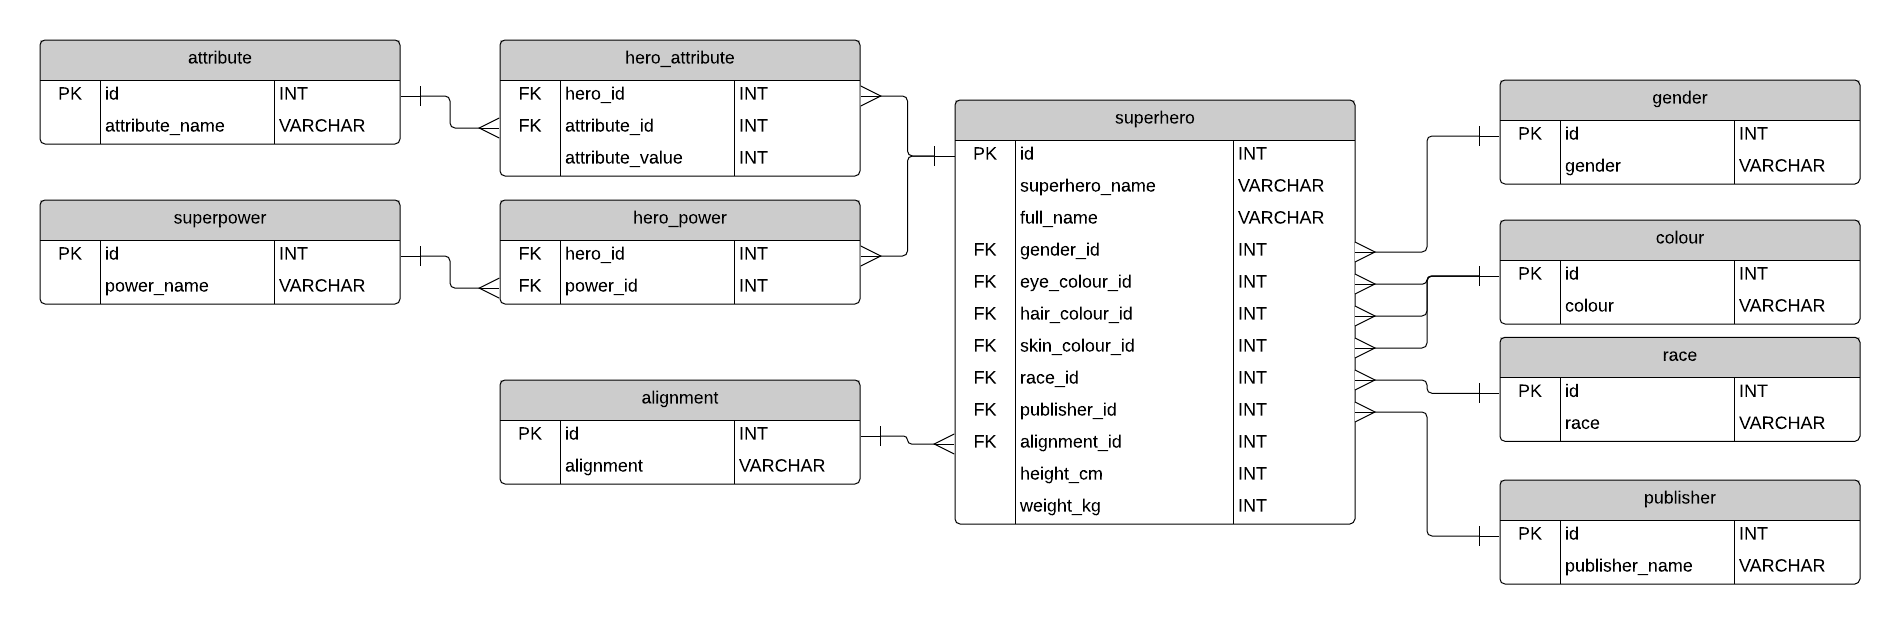
\includegraphics[width=\textwidth]{figures/erd}
 \caption{The Superhero Database E-R Diagram (available at \url{https://www.databasestar.com/sample-database-superheroes/}).}
 \label{fig:erd}
\end{figure}

The website \url{https://www.databasestar.com/} provides a rich collection of sample databases. One of them is the \textit{``Superhero''} database. You will read the documentation about it at \url{https://www.databasestar.com/sample-database-superheroes/}. See Figure \ref{fig:erd} for the E-R diagram of this database. To load the data into PostgreSQL, you will need to download three files:

\begin{enumerate}
  \item \href{https://drive.google.com/file/d/117RF0tbGk4LHhpcnBGr13Jl7C7GdUaB4/view?usp=drive_link}{\texttt{01\_reference\_data.sql}}.
  \item \href{https://drive.google.com/file/d/1j7lT45SjCtCo2Hc1fP5ej-Uopl0V1ZJR/view?usp=drive_link}{\texttt{02\_hero\_attribute.sql}}.
  \item \href{https://drive.google.com/file/d/1cV0cqxUjbCV1k67CPb-9wYkS_ymcF4Kq/view?usp=drive_link}{\texttt{03\_hero\_power.sql}}.
\end{enumerate}

Download the files and place them in the same folder. You must load the files in order, one after the other, in the same way we did in the last lab.

First, we will create a database named \texttt{heroes}:

\begin{minted}
[tabsize=4, obeytabs, frame=lines, framesep=2mm, baselinestretch=1.2, bgcolor=LightGray, fontsize=\footnotesize]{bash}
createdb heroes
\end{minted}

Next, we will connect to the database:

\begin{minted}
[tabsize=4, obeytabs, frame=lines, framesep=2mm, baselinestretch=1.2, bgcolor=LightGray, fontsize=\footnotesize]{bash}
psql heroes
\end{minted}

Now that we are in the PostgreSQL prompt, we will use the \textbackslash i command to load the files into our database. You will need to update the file paths accordingly.

First, we will load the \texttt{01\_reference\_data.sql} file:

\begin{minted}
[tabsize=4, obeytabs, frame=lines, framesep=2mm, baselinestretch=1.2, bgcolor=LightGray, fontsize=\footnotesize]{bash}
\i /path_to_files/01_reference_data.sql
\end{minted}

Then, we will load the \texttt{02\_hero\_attribute.sql} file:

\begin{minted}
[tabsize=4, obeytabs, frame=lines, framesep=2mm, baselinestretch=1.2, bgcolor=LightGray, fontsize=\footnotesize]{bash}
\i /path_to_files/02_hero_attribute.sql
\end{minted}

Finally, we will load the \texttt{03\_hero\_power.sql} file:

\begin{minted}
[tabsize=4, obeytabs, frame=lines, framesep=2mm, baselinestretch=1.2, bgcolor=LightGray, fontsize=\footnotesize]{bash}
\i /path_to_files/03_hero_power.sql
\end{minted}

And you're done! Let's read a transcript of a podcast discussing the database. You can read it in \href{https://drive.google.com/file/d/1alLbRweqVIJvVZvG_fIwm-Fz41NlRCfp/view?usp=drive_link}{English} or \href{https://drive.google.com/file/d/1XjZgzHFuMucLsprRc5Rx5nP4L2idfPE1/view?usp=drive_link}{Spanish}, and try out the SQL examples found there.

\section{Independent Work}
Let's see what we can learn from the \texttt{superhero} database. You are asked to answer the following queries\footnote{Use only JOIN variants in your answers.}:

\begin{enumerate}
  \item What is Magneto's full name?
  \item Retrieve each superhero’s name along with the publisher’s name.
  \item Display the name, full name, and gender of \textit{supervillains}. We define a \textit{supervillain} as a superhero with a ``Bad'' alignment.
  \item Based on gender, which group has more superpowers? Show the total for each category.
  \item List the superheroes who are the most diverse, meaning those who have different eye, hair, and skin colors. Display all colors along with the superhero's name.
  \item Display the list of superheroes who do not have any attributes at all. Hint: Use a \texttt{LEFT JOIN} and look for \texttt{\textbf{null}} values.
  \item True or False: Does `Marvel Comics' have more ``Good'' superheroes than `DC Comics'?
  \item What is the average height and maximum weight of characters published by `Dark Horse Comics'? Do not take into account any \texttt{\textbf{null}} or $0$ values in the calculation.
  \item Who is stronger: Superman or Goku? We will measure strength using the following formula:
  $$
    \text{strength} = \text{count\_of\_attributes} + 2 \times \text{count\_of\_powers}
  $$
  \item Shows all of the superheroes and the sum of their attributes, including those with no attributes.
  \item This time, you are asked to propose \textbf{TWO} queries using any (different) variant of \texttt{JOIN} and solve them using \texttt{SQL} on your own.
\end{enumerate}

For each query, you must present the \texttt{SQL} code and the query result (either copy-pasted or as a screenshot). We expect you to submit a well-structured report in PDF format, containing the requested information from the previous sections. Additionally, include the \texttt{SQL} code with the answers to the queries in a ZIP file via Brightspace. The submission deadline is \textbf{September 3, 2025}.

\vspace{5mm}
Happy Hacking! \includesvg[width=4mm]{figures/sunglasses}

\end{document}
